\chapter{Benchmarking and Result}

\minitoc

\section{Fine Tuning the Deep Learning Models}

On top of the five main dataset of size $> 20k$, DeepPrime additionally has 18 datasets of size $\sim5k$, which were used to fine tune the model for better generalizability. As a result, for a more thorough comparison between the models, the same fine tuning process was conducted on all deep learning models.

To fine tune the models, the same hyperparameters during the original training were used, except for the learning rate, which was lowered to $1e^{-3}$ for the fine tuning to accommodate the smaller dataset size. On top of that, the NRCH versions of prime editors were used in some of the small datasets, which contains optimized SpCas9 proteins that can accommodate NRCH PAMs (N = A, T, C, G; R = A, G; H = A, C, T) \cite{millerContinuousEvolutionSpCas92020}. The pam matching function was thus updated to accommodate the extra PAMs when determining if the protospacer adjacent motifs were disrupted during the edit.

The models trained on the DeepPrime HEK293T PE2 dataset were selected for fine tuning, as DeepPrime has the largest dataset and was thus most likely to have enough examples for the deep learning models to learn the underlying motifs. To preserve the sequence features acquired on the DeepPrime dataset, the sequence processing layers were frozen, leaving only the biological feature processing MLP and the final meta learner MLP to be trained. The models were trained for at most 300 epochs for each fold, and the model with the best validation loss was saved for evaluation.

% TODO: add references to the section and appendix after including the results

\section{Performance on All Datasets}

\begin{figure}
    \centering
    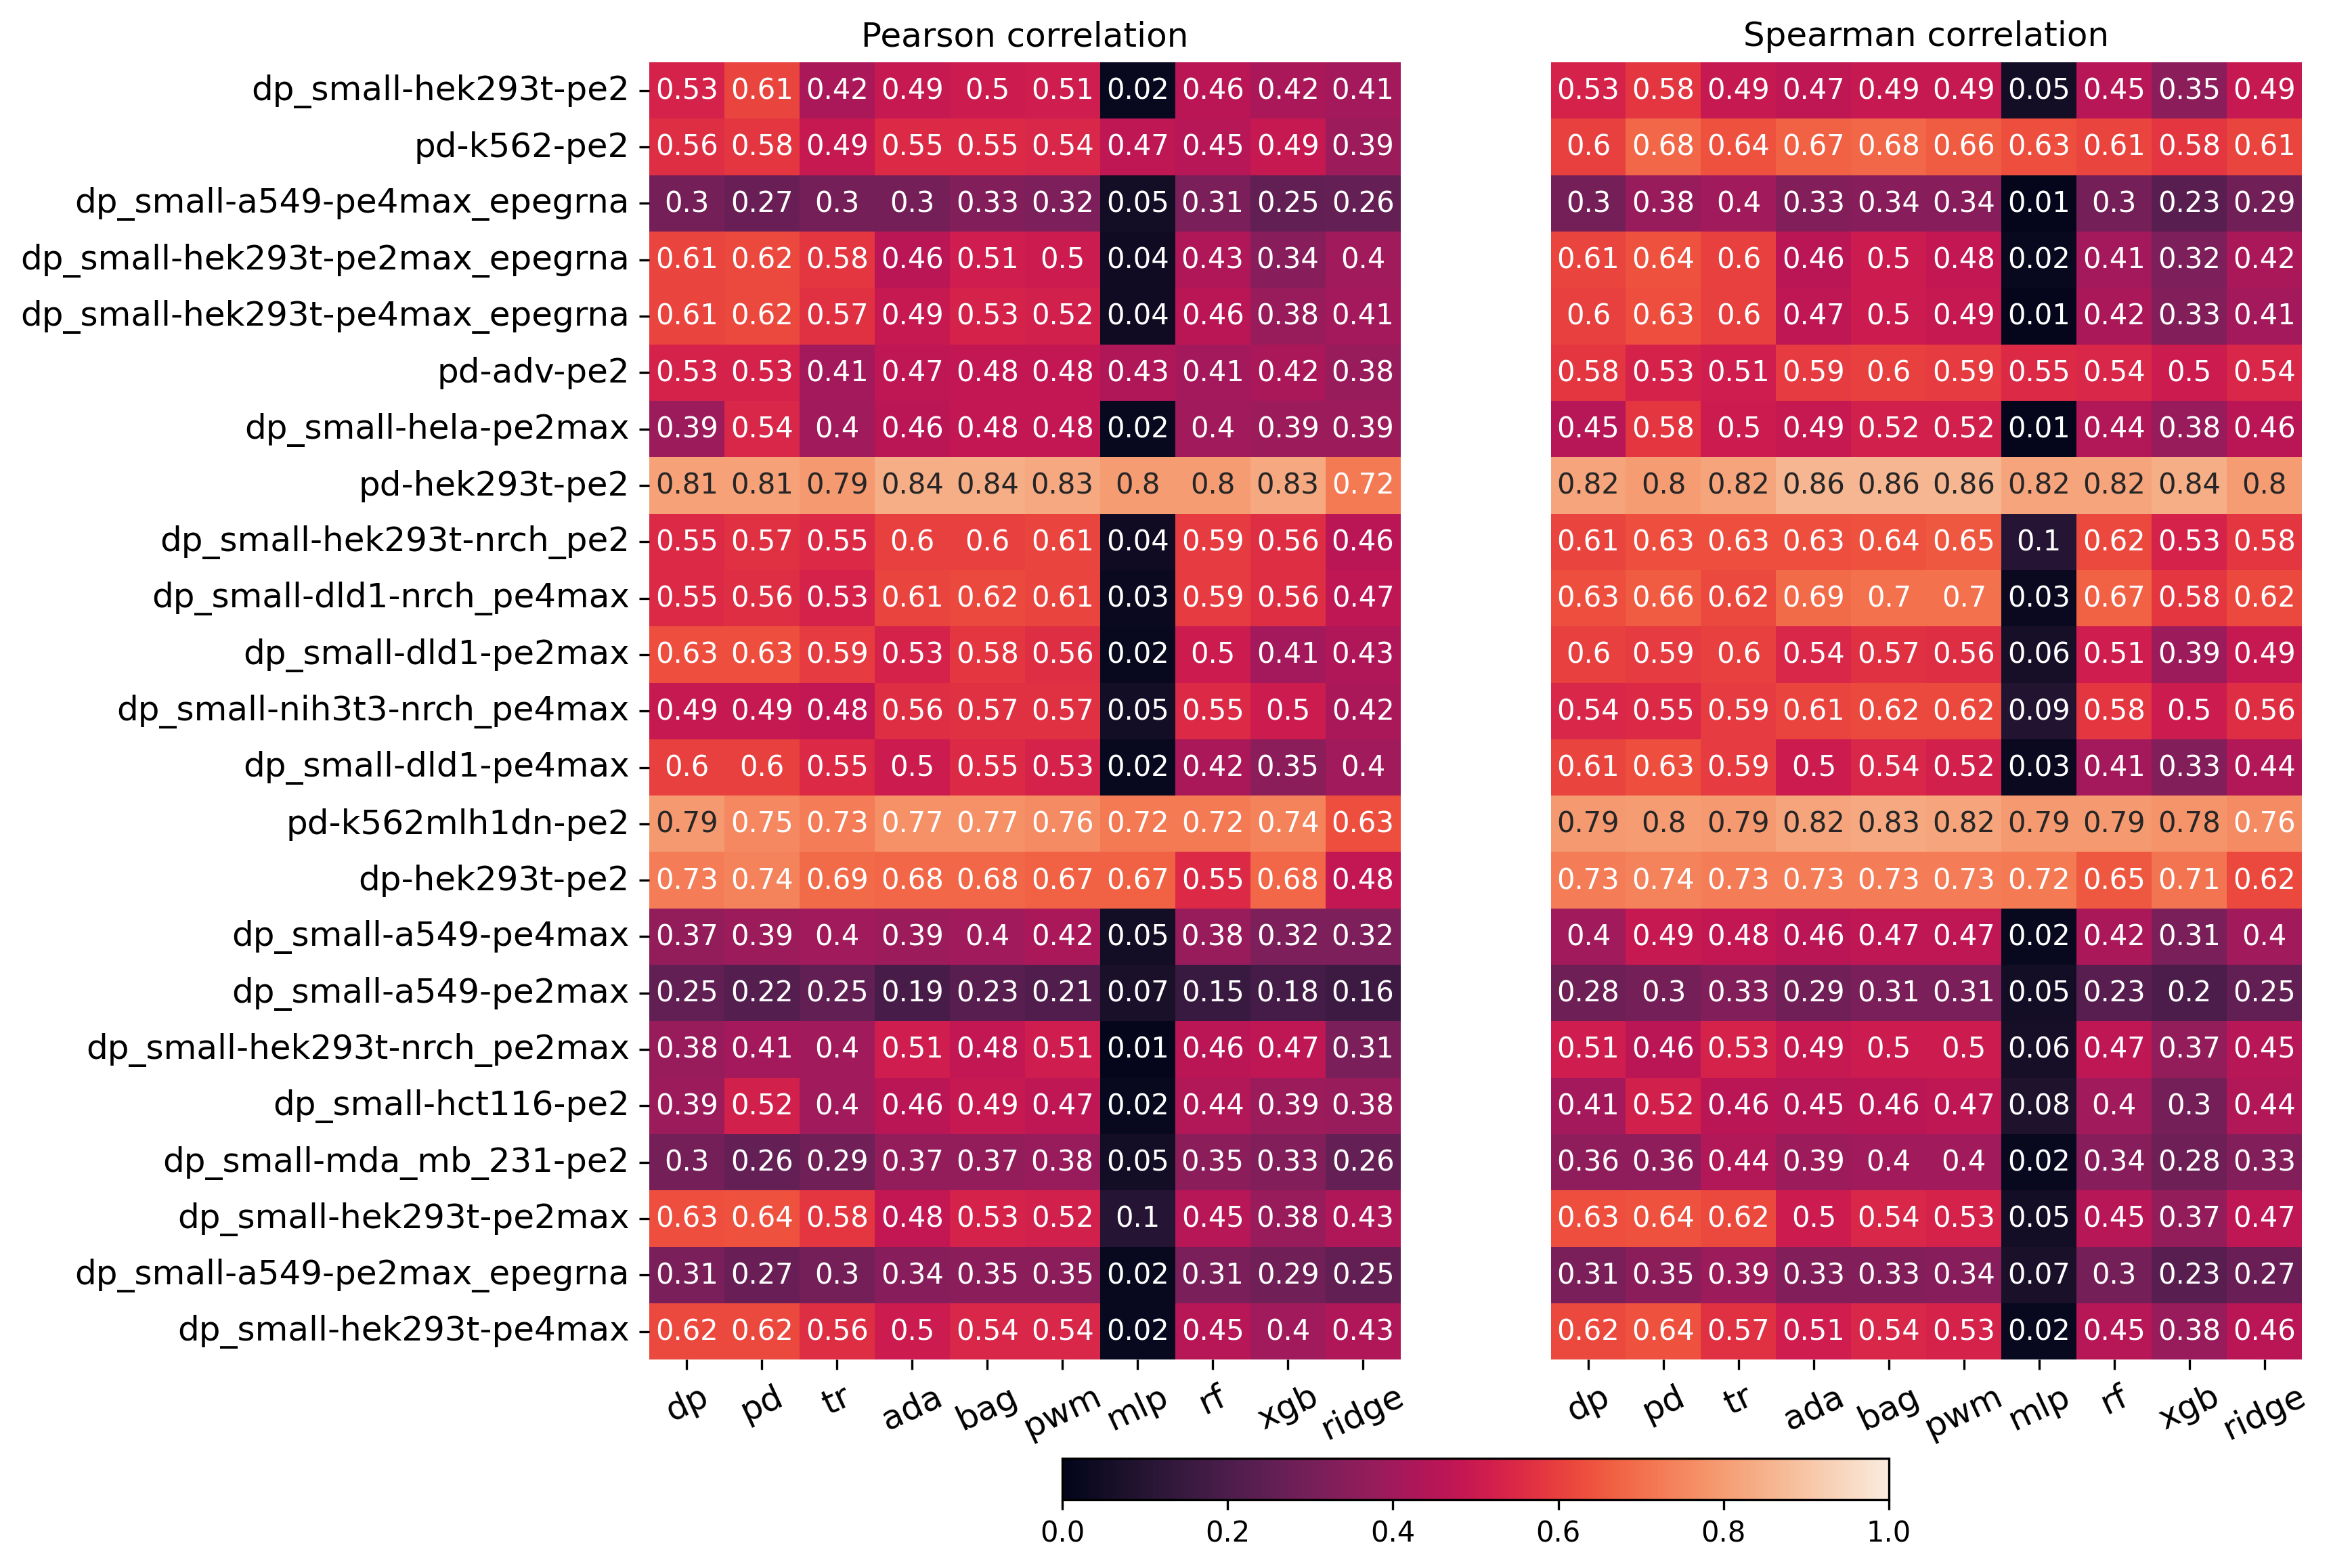
\includegraphics[width=\textwidth]{all_models_performance.png}
    \caption[Performance of the models on all datasets]{Performance of the deep learning models on all datasets. The x-axis represents the model name, while the y-axis represents the datasets used for training and testing. The mean performance of the models across five folds is shown in the heatmap, with brighter colours indicating higher Pearson or Spearman correlation.
    As mentioned in \autoref{sec:datasets}, the datasets are named in the format of `data source - cell line - prime editor'. 
    
    There were three data sources involved during benchmarking - DeepPrime (dp), PRIDICT (pd), and DeepPrime Small (dp\_small, $\sim5k$ examples). At the same time, the cell line and prime editors' names are self-explanatory. 
    
    Four models in total were produced in this study - the transformer based model (tr), the power weighted mean ensemble (pwm), the bagging ensemble (bag), and the adaboost ensemble (ada). Their performances are highlighted in the heatmap with the red bounding boxes.
    They were compared with the two state of the art deep learning solutions, DeepPrime (dp) and PRIDICT (pd). The datasets where any of the models trained in this study significantly outperformed both DeepPrime and PRIDICT are marked with a blue bounding box (performance across five folds, $p<0.05$, paired t-test).
    }
    \label{fig:performance}
\end{figure}

As discussed in \autoref{sec:ensemble}, all three ensemble models were able to significantly outperform the base learners on the PRIDICT HEK293T PE2 dataset. Thus, power weighted mean ensemble, bagging and adaboost were trained using the full ensemble (including the deep learning models) on all available datasets alongside the transformer model to evaluate their performance against the base learners, as well as DeepPrime and PRIDICT.

Unfortunately, the transformer model failed to significantly outperform DeepPrime and PRIDICT on any of five main datasets, with lower Pearson's $r$ and similar Spearman's $\rho$. Additionally, when compared with the conventional machine learning models' performance in \autoref{fig:conventional_ml_models_performance}, only marginal improvement was observed over the MLP model that makes up part of the transformer model in the DeepPrime dataset ($r$ of 0.69 vs 0.67), and no improvement was observed in the PRIDICT dataset. This indicates that the transformer model may not have contributed significantly to the outcome, and the performance was mainly driven by the MLP model. 

However, it did outperform DeepPrime and PRIDICT on two of the DeepPrime small datasets (A549 PE2-max and A549 with PE2-max using engineered pegRNA (epegRNA)) in terms of Spearman correlation, but not Pearson correlation. The consistently better performance on A549 PE2-max dataset may suggest that the motifs learned by the transformer model are especially useful for this configuration. 

The three ensemble methods showed similar performance with each other across all datasets, with bagging and adaboost often marginally outperforming the power weighted mean ensemble. They significantly outperformed PRIDICT and DeepPrime on two of the PRIDICT datasets in terms of Pearson or Spearman correlation (HEK293T PE2 and K562MLH1dn PE2), as well as on two of the DeepPrime small datasets. One of the most significant boost in performance was observed on the PRIDICT HEK293T PE2 dataset, where the tuning of AdaBoost and Bagging ensemble models' hyperparameters was performed. This hints that the ensemble methods, especially AdaBoost and Bagging, can be sensitive to the dataset size and composition, and may benefit from retuning on each dataset.


\section{Performance on Individual Editing Types}

On top of the overall performance, the performances of the models on individual editing types were also evaluated on the five main datasets to understand the models' ability to handle different types of mutations. 

\begin{figure}
    \centering
    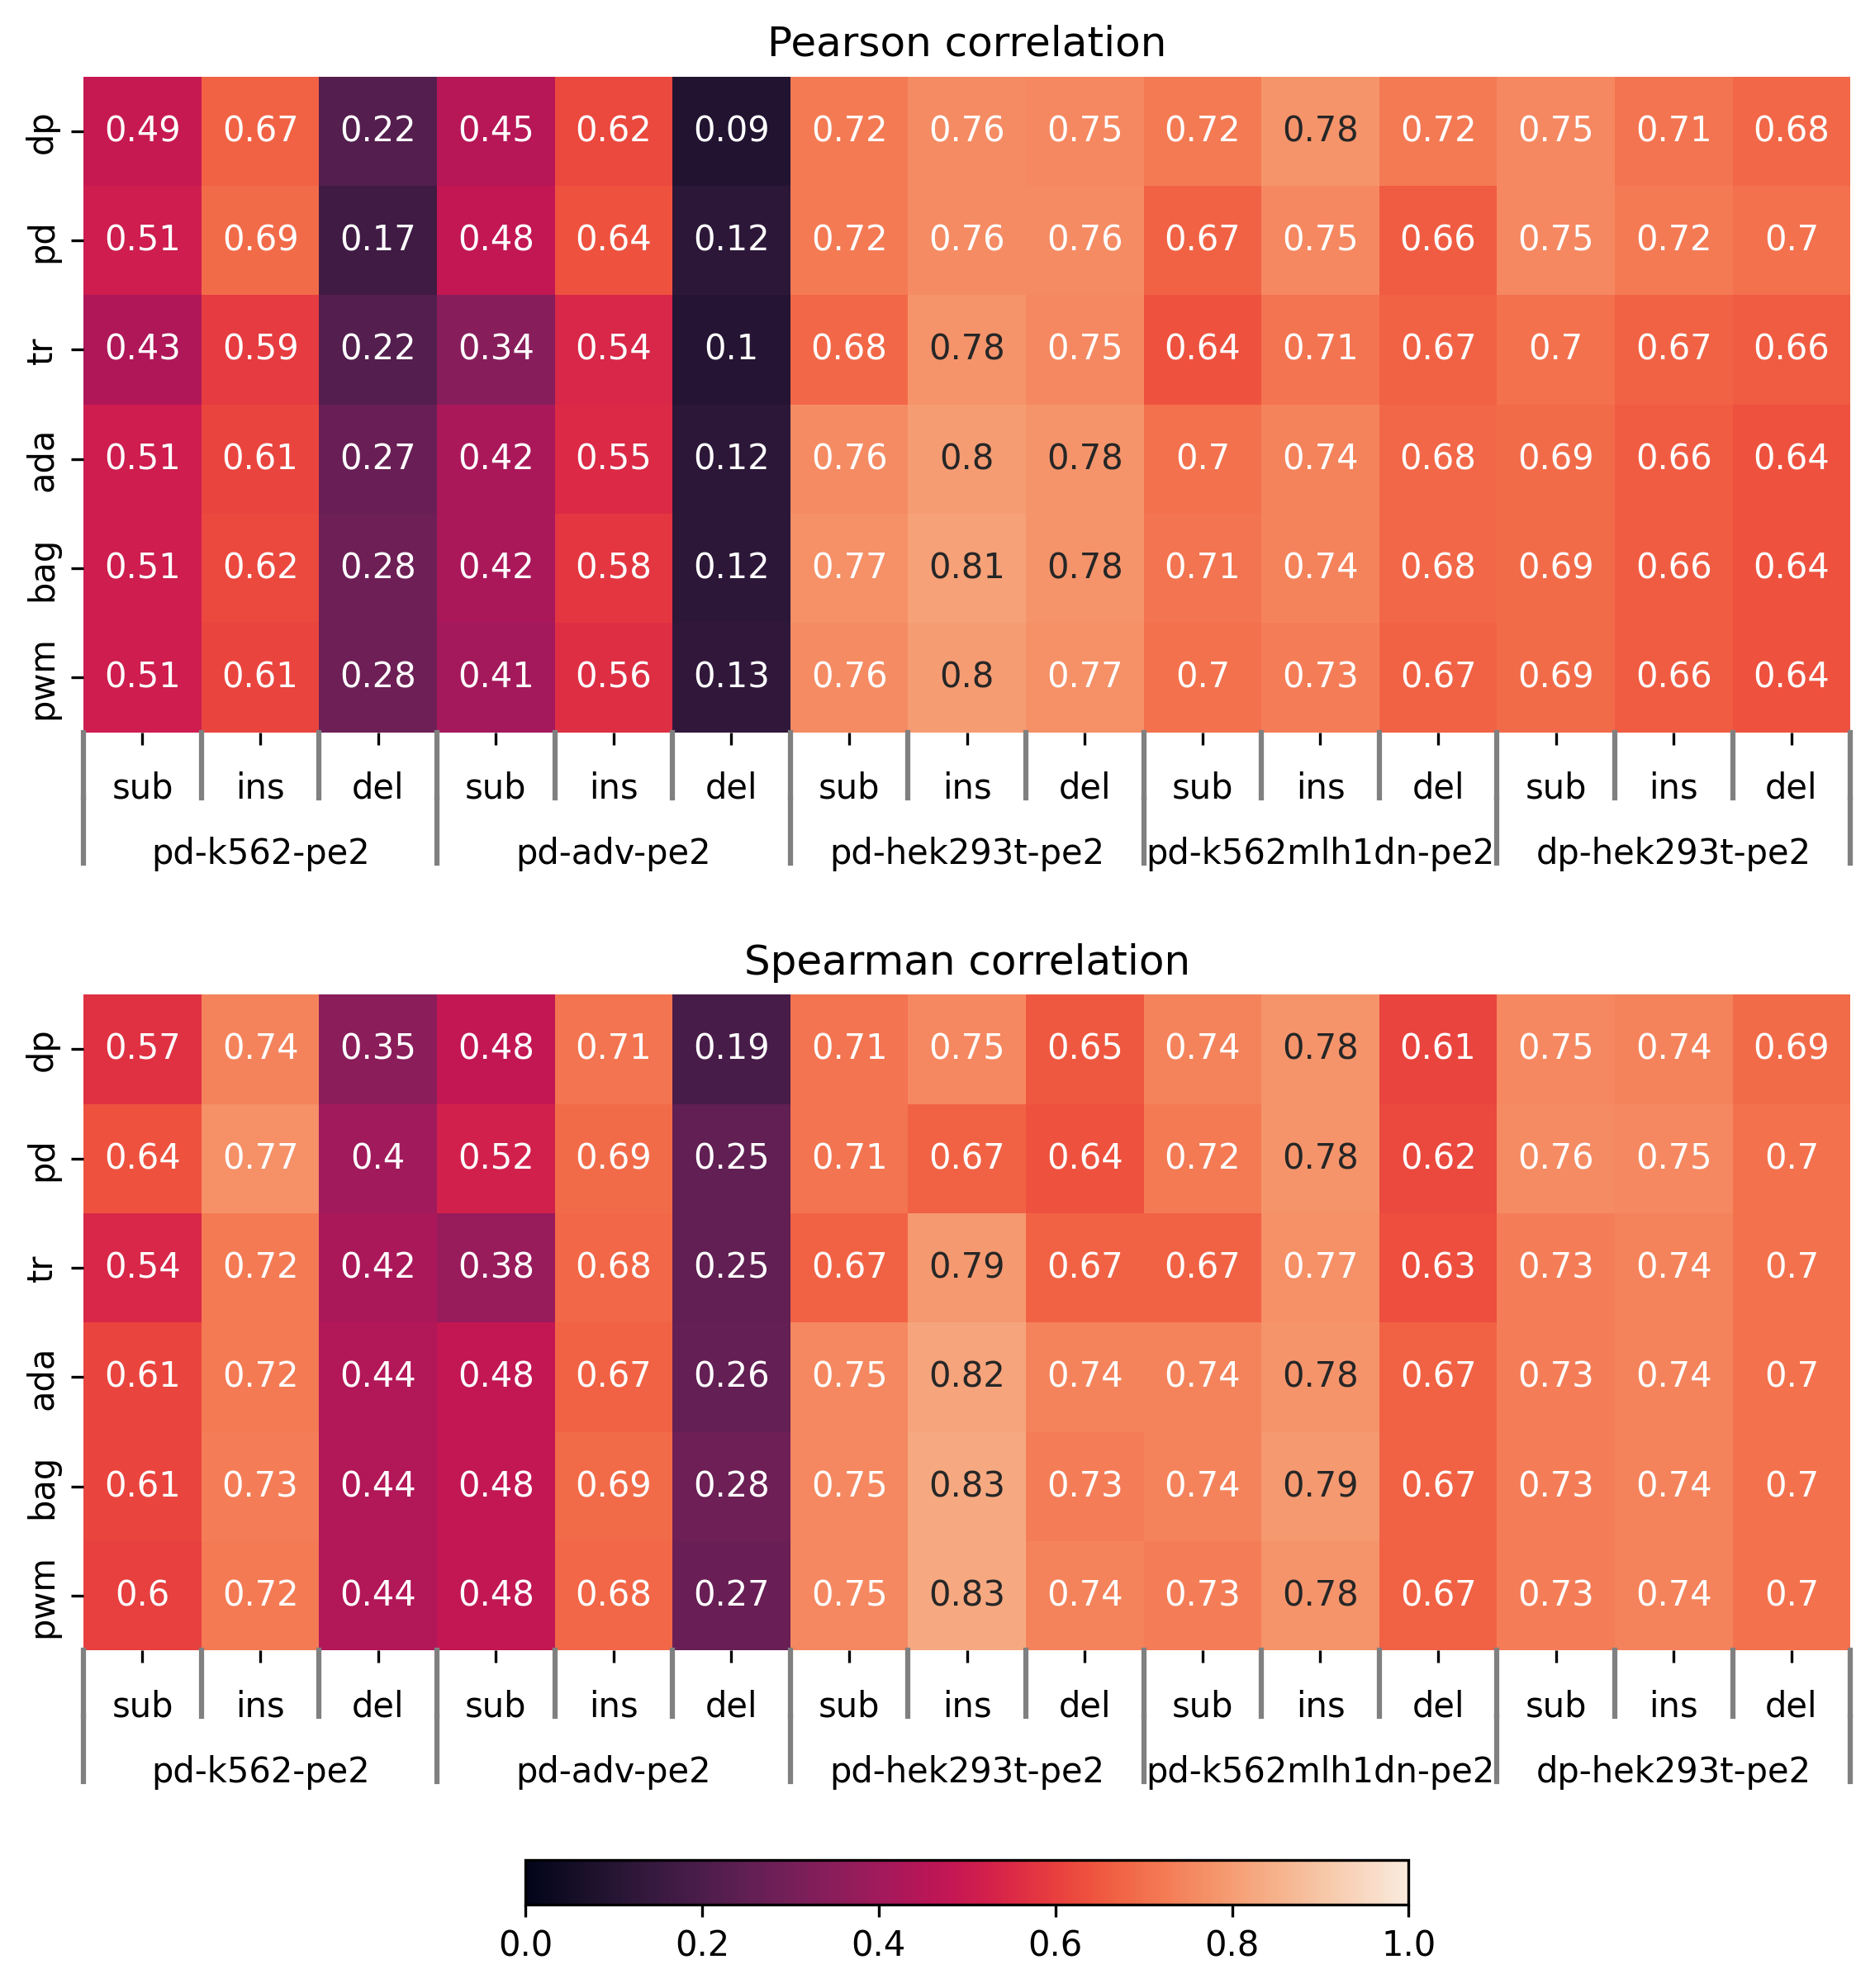
\includegraphics[width=0.8\textwidth]{all_models_performance-edits.png}
    \caption[Performance of the models on individual editing types]{Performance of the deep learning and ensemble models on individual editing types. Contrary to \autoref{fig:performance}, the x-axis now illustrates the name of the dataset and the corresponding edit type subset (sub[stitution], ins[ertion], [deletion]), while the y-axis represents the model names. Similar to \autoref{fig:performance}, the mean performance of the models across five folds is shown in the heatmap, with brighter colours indicating higher pearson or spearman correlation. The only dataset where the models trained in this study achieved statistically significant improvement over DeepPrime and PRIDICT was the PRIDICT HEK293T PE2 dataset, marked with a blue bounding box.}
    \label{fig:performance_edits}
\end{figure}

Illustrated in \autoref{fig:performance_edits}, the performances of transformer model on individual edit types were mostly consistent with the overall performances in terms of Pearson's $r$. The transformer model falls short of the performance of PRIDICT and DeepPrime on all edit types and datasets other than PRIDICT HEK293T PE2, where it marginally outperformed PRIDICT on insertion examples.

At the same time, although the transformer model was on par with PRIDICT and DeepPrime when evaluated with Spearman's $\rho$ on overall data, the relative performances of the models were not consistent across different mutations. The transformer model was often on par or can marginally outperform PRIDICT and DeepPrime when predicting insertion and deletion efficiency. However, the performance of the transformer model on substitution examples was consistently lower than PRIDICT and DeepPrime.

The relative performances of the ensemble models with DeepPrime and PRIDICT were more complex and varied more substantially across different datasets, possibly due to their sensitivity to hyperparameters mentioned in the \autoref{sec:ensemble}. 

The ensemble models had slightly lower Pearson and Spearman performance on the substitution and insertion examples of the PRIDICT K562 dataset, but noticeably outperformed PRIDICT and DeepPrime on the deletion examples. The same was true for the PRIDICT Adv dataset when evaluated with Spearman's $\rho$, while only similar performance for the deletion examples was observed when evaluated with Pearson's $r$.

Pronounced improvement on the deletion examples was also observed on the PRIDICT K562MLH1dn PE2 dataset, but in this case, the ensemble models were able to match the performance of PRIDICT and DeepPrime on the substitution and insertion examples.

Finally, on the PRIDICT HEK293T PE2 dataset, the ensemble models significantly outperformed PRIDICT and DeepPrime on all edit types ($p<0.05$, paired t-test across five folds), while the opposite was true for the larger DeepPrime dataset.

\section{Attention Analysis}
\label{sec:attention_analysis}

\begin{figure}
    \centering
    \subfigure[Substitution]{
        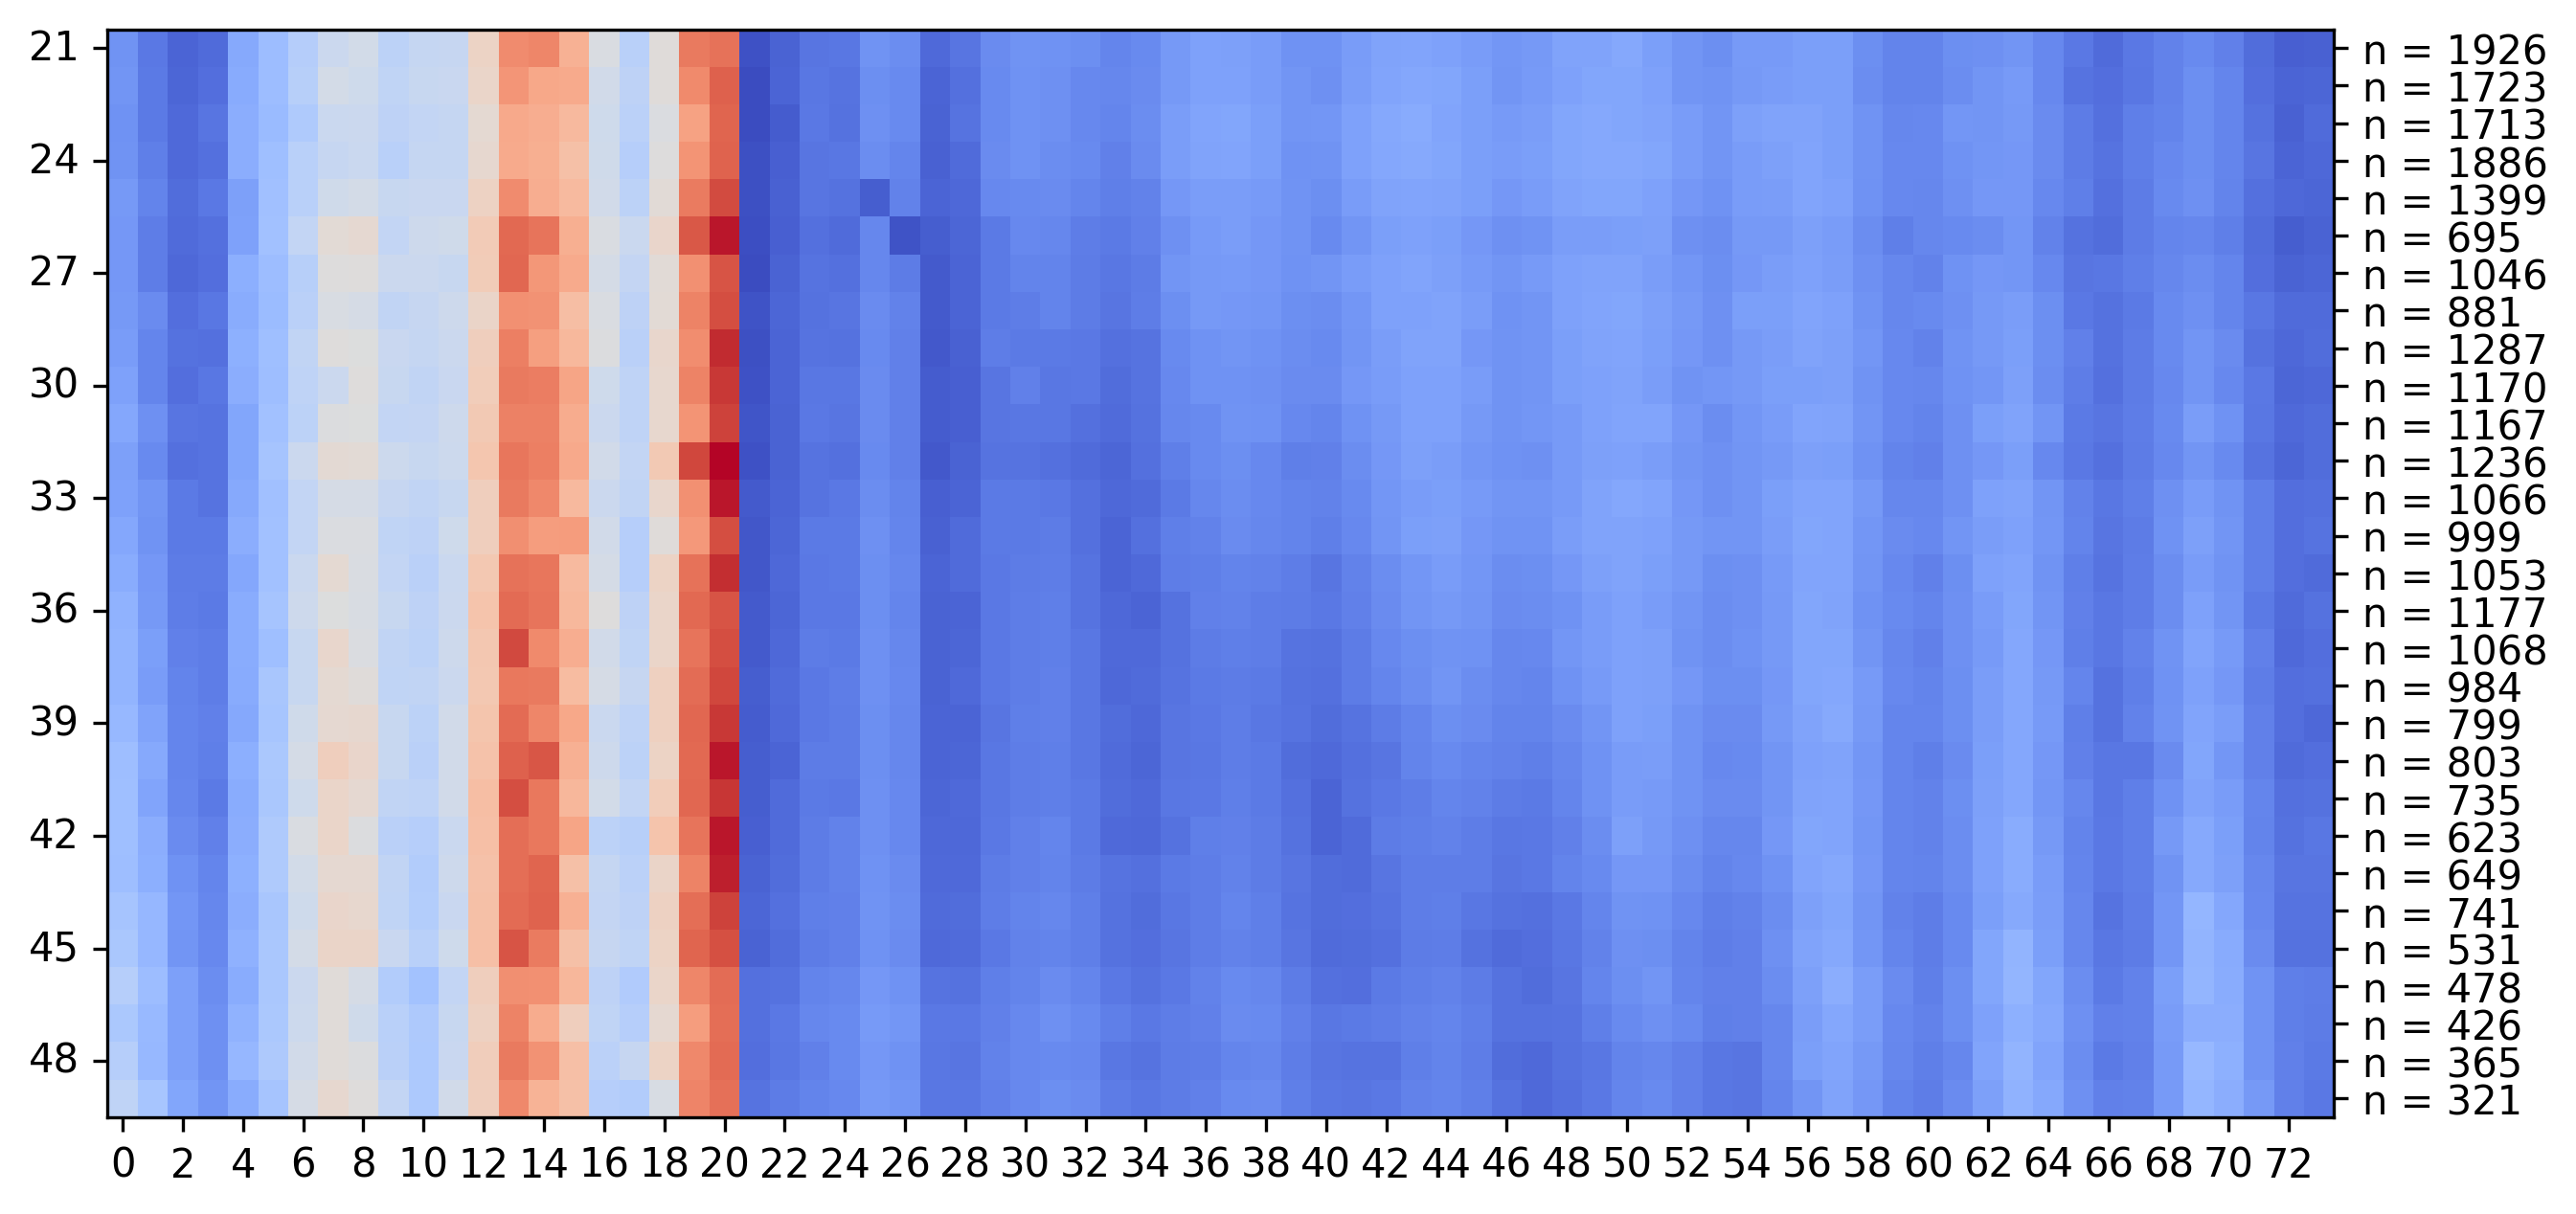
\includegraphics[width=0.85\textwidth]{dp-hek293t-pe2-transformer-only-attention-replace-1bp.png}
        \label{fig:attention_insertion}
    }
    \subfigure[Insertion]{
        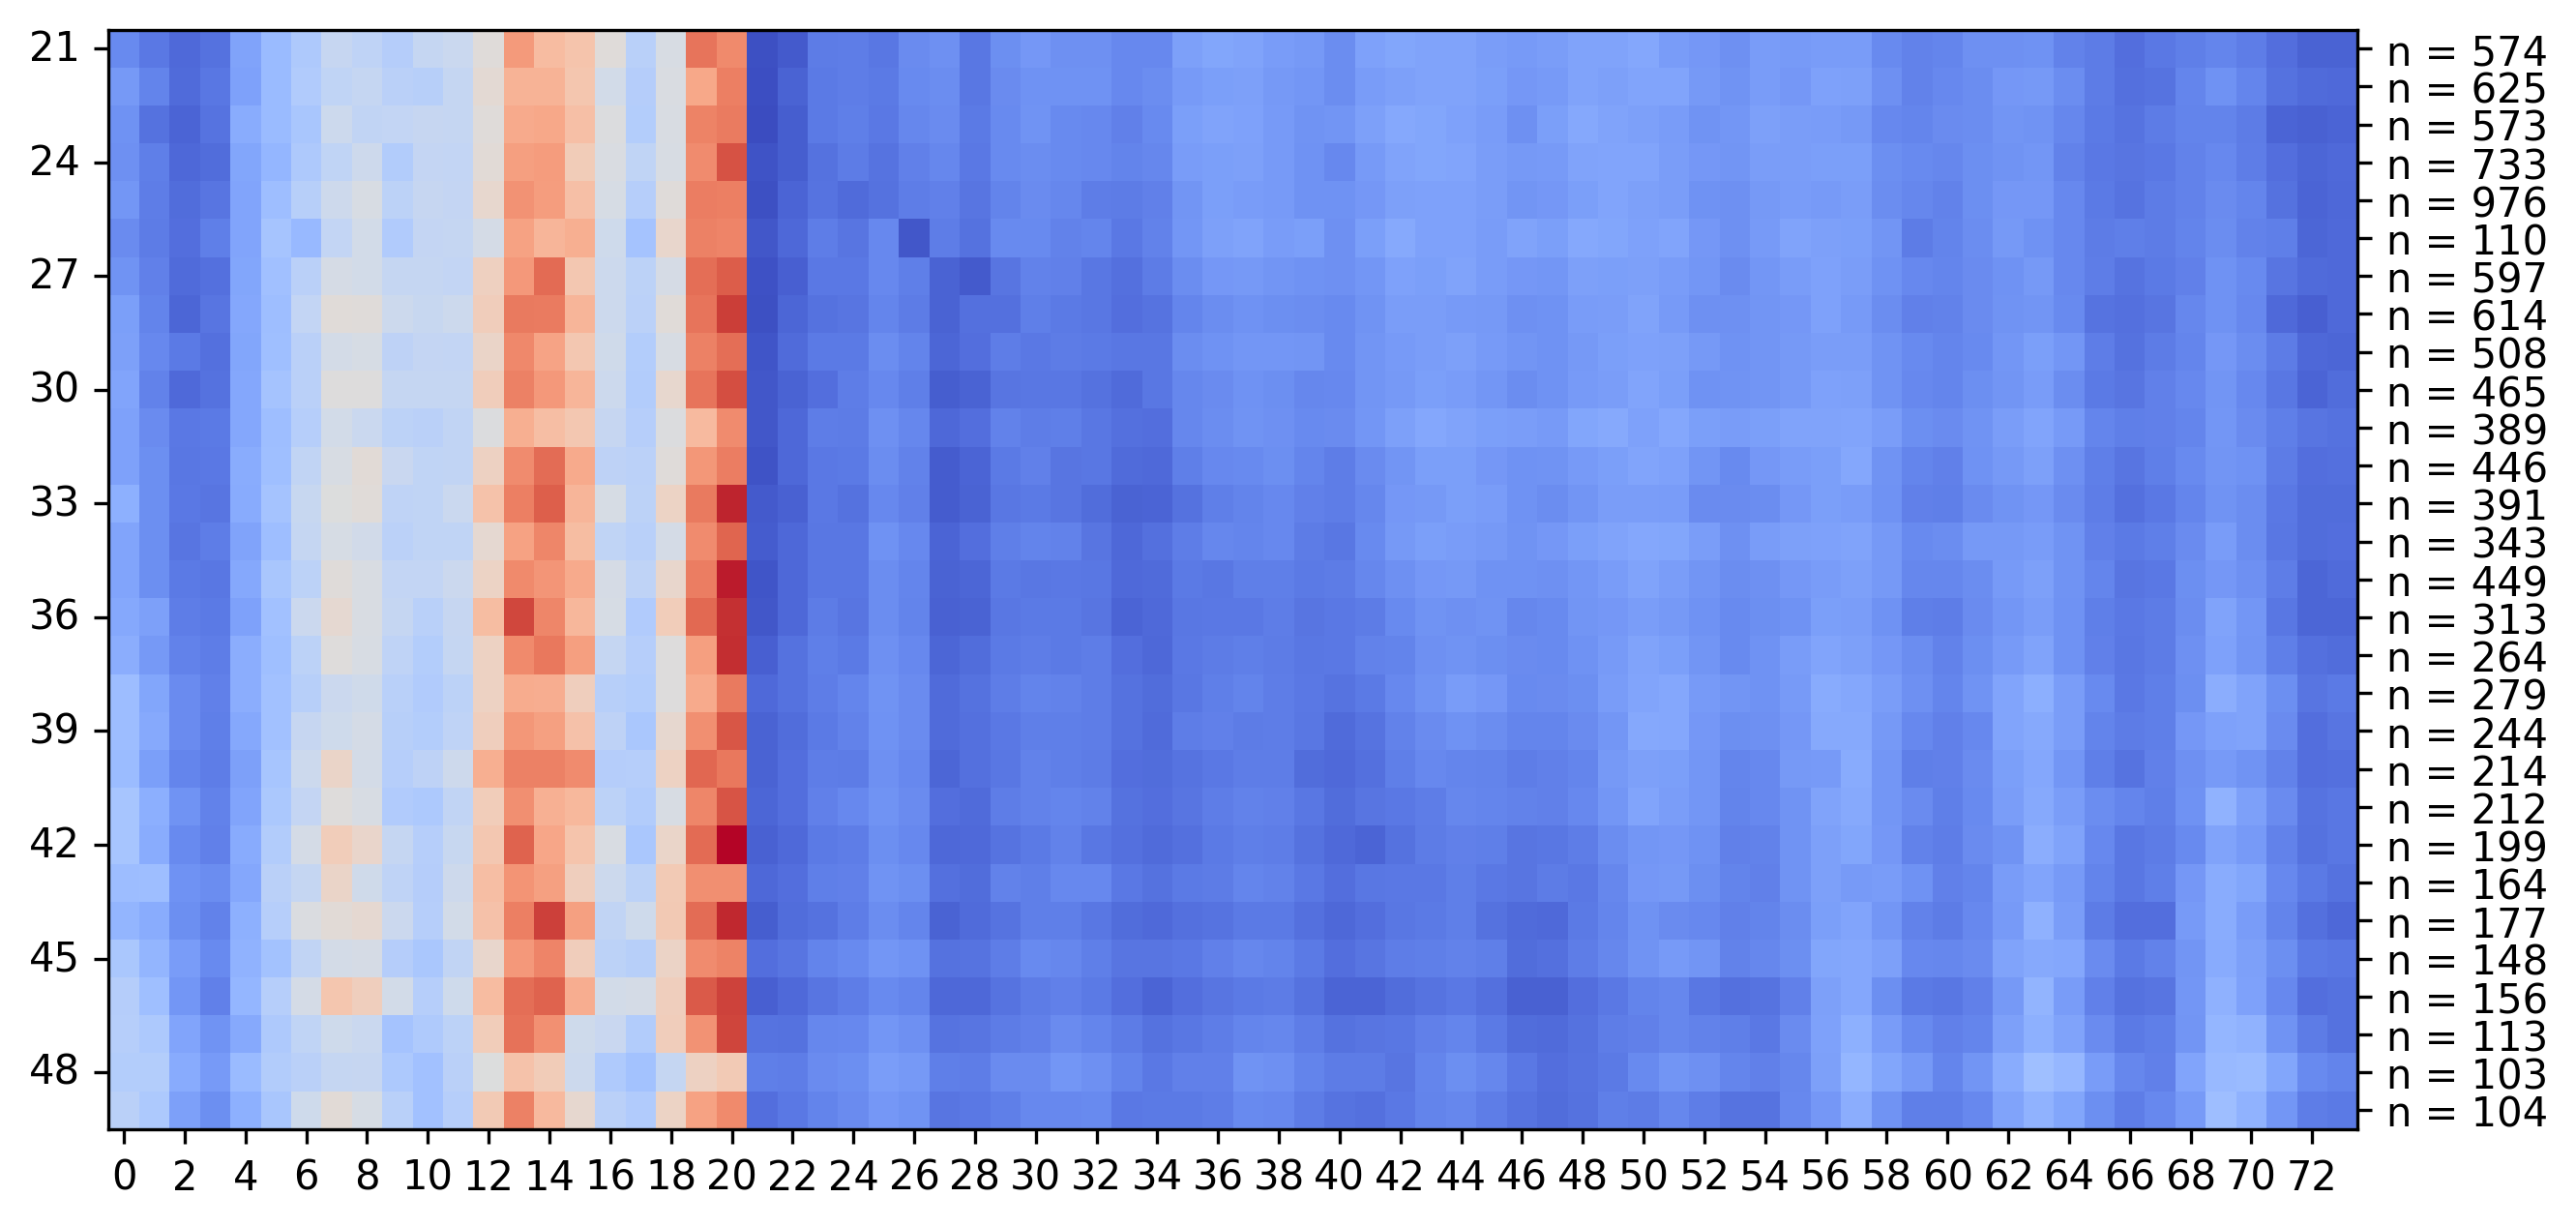
\includegraphics[width=0.85\textwidth]{dp-hek293t-pe2-transformer-only-attention-insertion-1bp.png}
        \label{fig:attention_substitution}
    }
    \subfigure[Deletion]{
        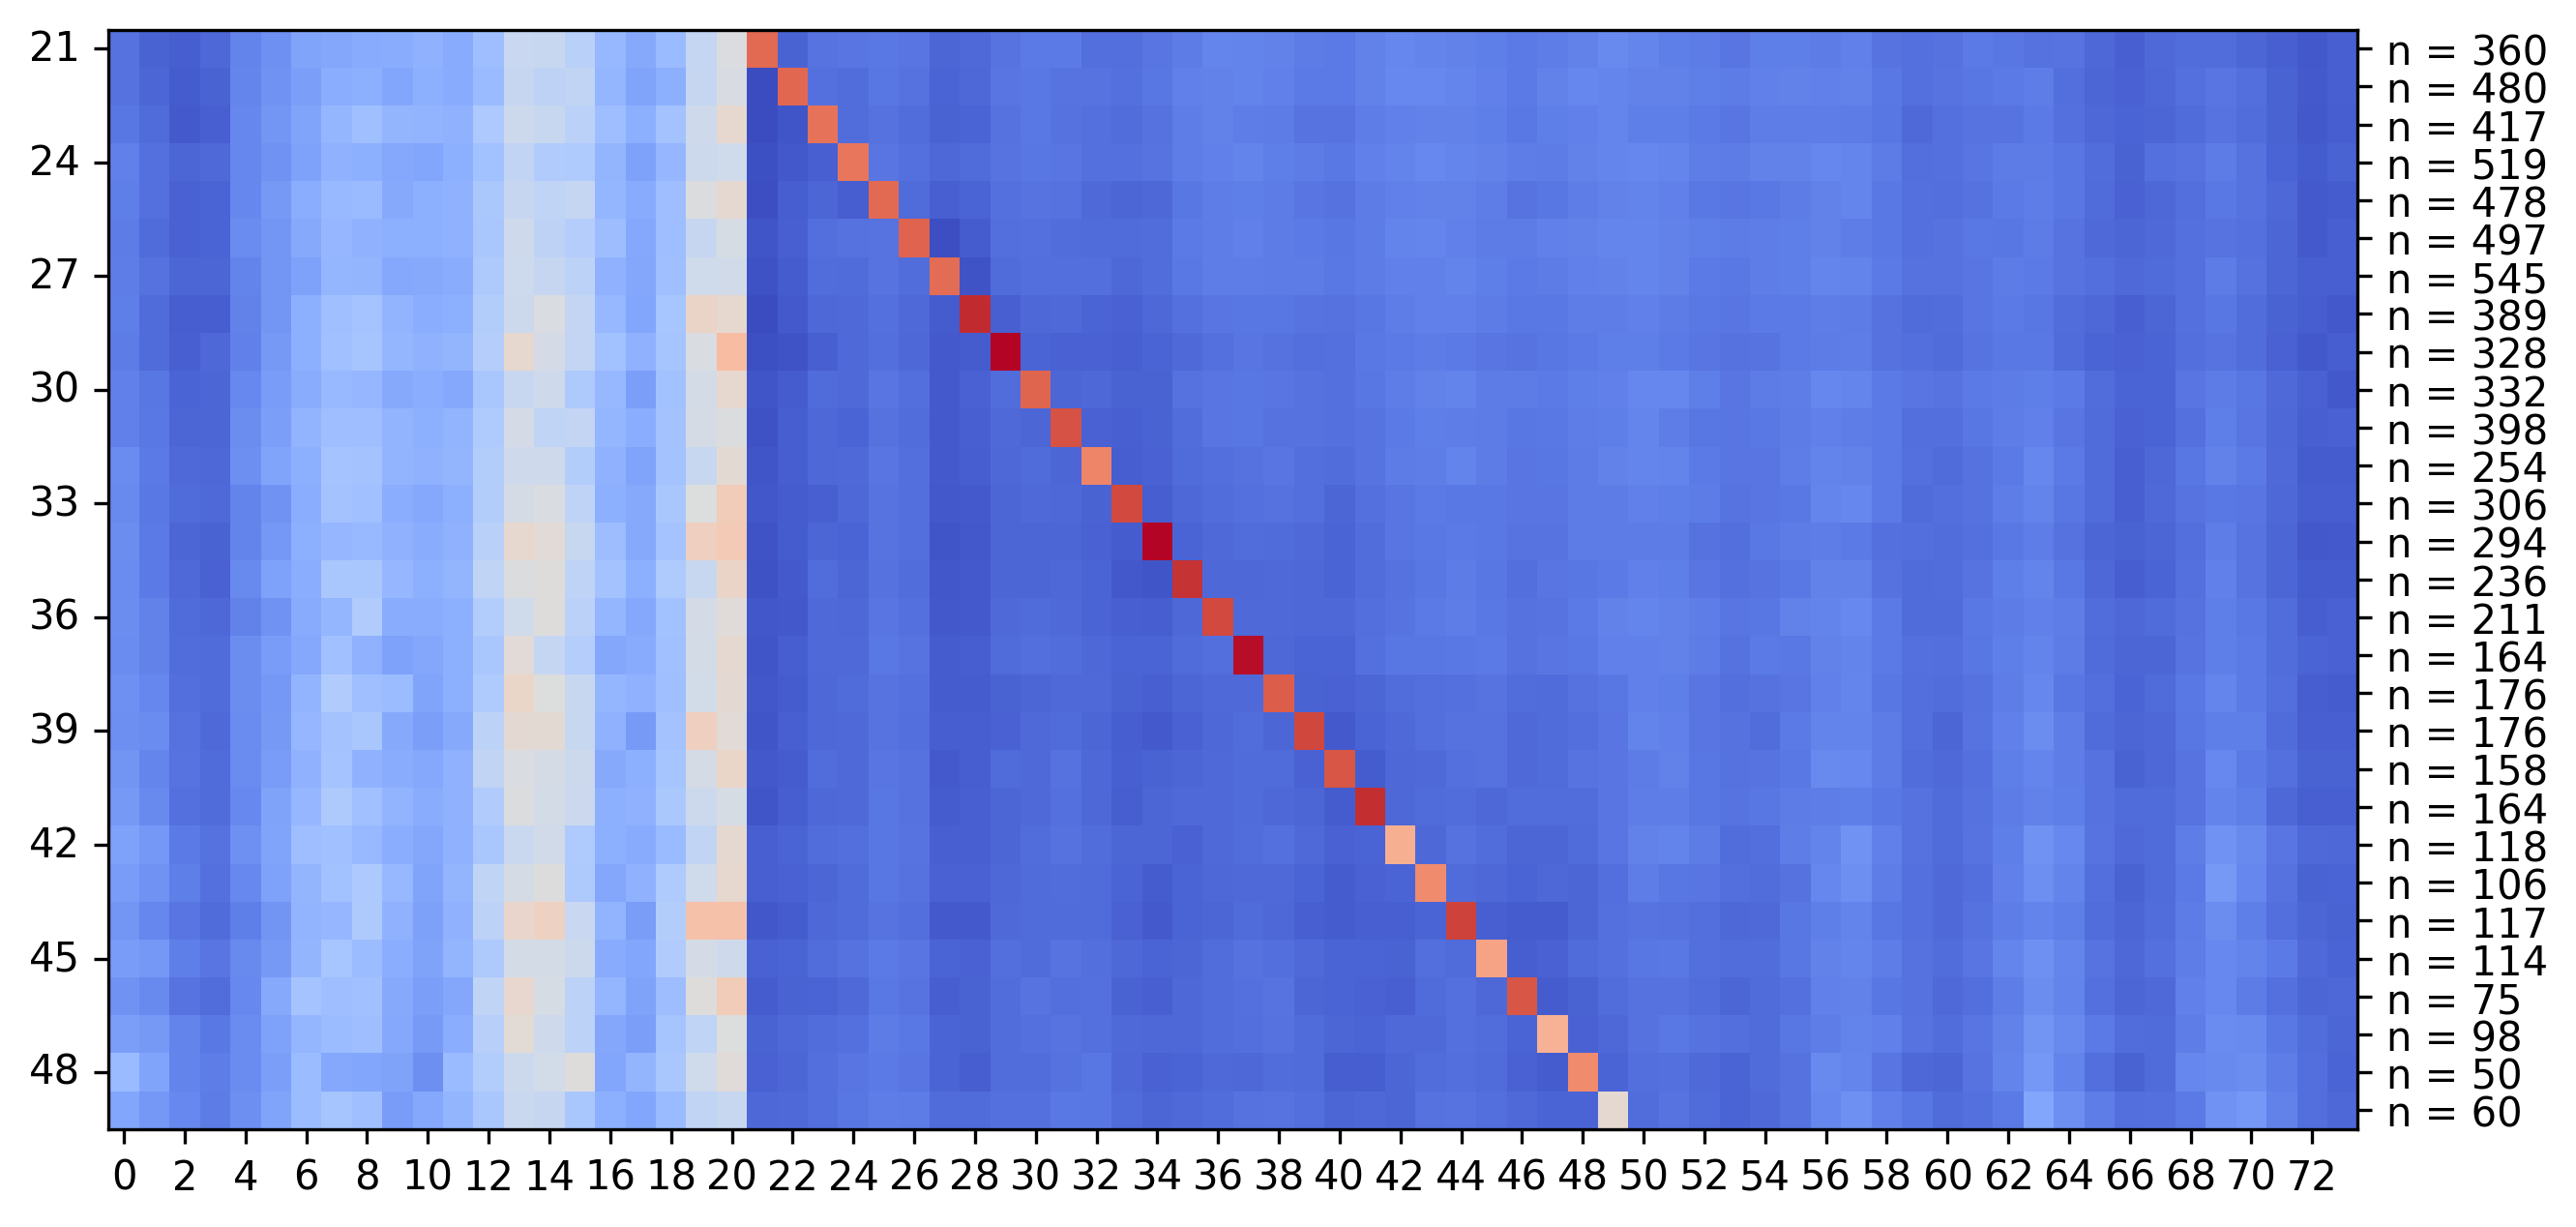
\includegraphics[width=0.85\textwidth]{dp-hek293t-pe2-transformer-only-attention-deletion-1bp.png}
        \label{fig:attention_deletion}
    }
    \caption[Attention weights for the DeepPrime model trained on the HEK293T-PE2 dataset]{Attention weights of length 1 edits for the DeepPrime model trained on the HEK293T-PE2 dataset. The x-axis represents the position of the transformer output token, the y-axis indicates the edit position. Red colour indicates higher attention weights, while blue represents lower attention weights. The example size for each edit location is shown on the right in the format of `n=number of examples'.}
    \label{fig:attention}
\end{figure}

A significant advantage of the attention based methods is their interpretability. The attention mechanism allows the model to focus on specific parts of the input data using the attention weights, which can be visualized to help understand some of the model's decision making process. 

In this architecture, the most informative and interpretable attention weights are the feature embedding attention weights at the final layer of the transformer model, pooling all token embeddings into a single vector of size token embedding (6) by attributing different weights to each token position. 

For better clarity, the examples were grouped together by their mutation types and lengths so that the edit positions can be easily identified and compared. The attention weights for edits at the same position were aggregated to show the overall importance of the position in the editing efficiency prediction.

The model trained on the biggest DeepPrime dataset was first tested, as the transformer model has the greatest chance of learning the underlying motifs influencing the editing efficiency in the data. Starting with the edits of length 1, the attention weights were visualized for the substitution, insertion, and deletion, shown in \autoref{fig:attention}. 

For both 1-bp substitution and insertion, the attention weights were the highest from around the start of the protospacer location (location 4) to the nick position (location 20, also where the PBS ends). This may be an indication that the model considers the composition of the PBS as an important feature for the editing efficiency prediction. Additionally, one of the hot spots for the attention weights was the protospacer location 13 to 17. This is highly consistent with the finding in \autoref{sec:determinants} that the nucleotides at protospacer positions 13 to 17 are important features for the editing efficiency prediction.

Meanwhile, for deletion, the attention weights were the highest at the edit position. The cross attention output of the edit position for deletion was dominated by the encoder output, as the self-attention weights for the mutated sequence at edit position were masked out to be zero. As a result, this is a possible indication that the model considers the base to delete as an important feature for the deletion operations.

\begin{figure}
    \centering
    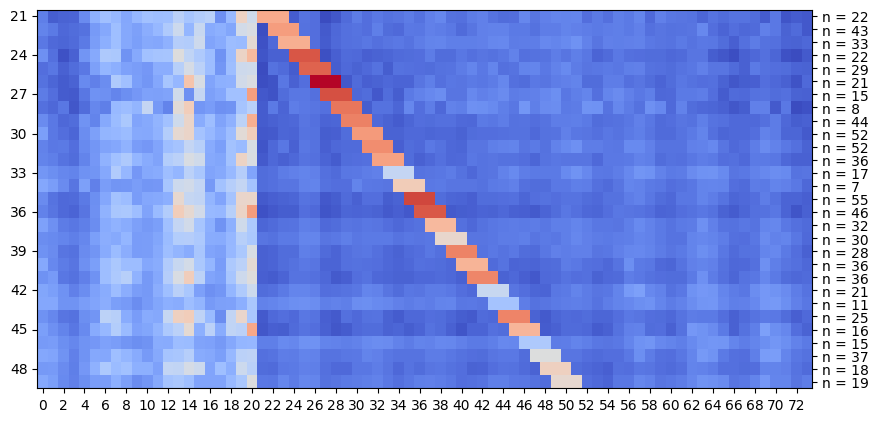
\includegraphics[width=0.85\textwidth]{dp-hek293t-pe2-transformer-only-attention-deletion-3bp.png}
    \caption[Attention weights for 3-bp deletion of the DeepPrime model trained on the HEK293T-PE2 dataset]{Similar to \autoref{fig:attention}, attention weights of length 3 deletion for the DeepPrime model trained on the HEK293T-PE2 dataset.}
    \label{fig:attention_deletion_3bp}
\end{figure}

\begin{figure}
    \subfigure[Replacement]{
        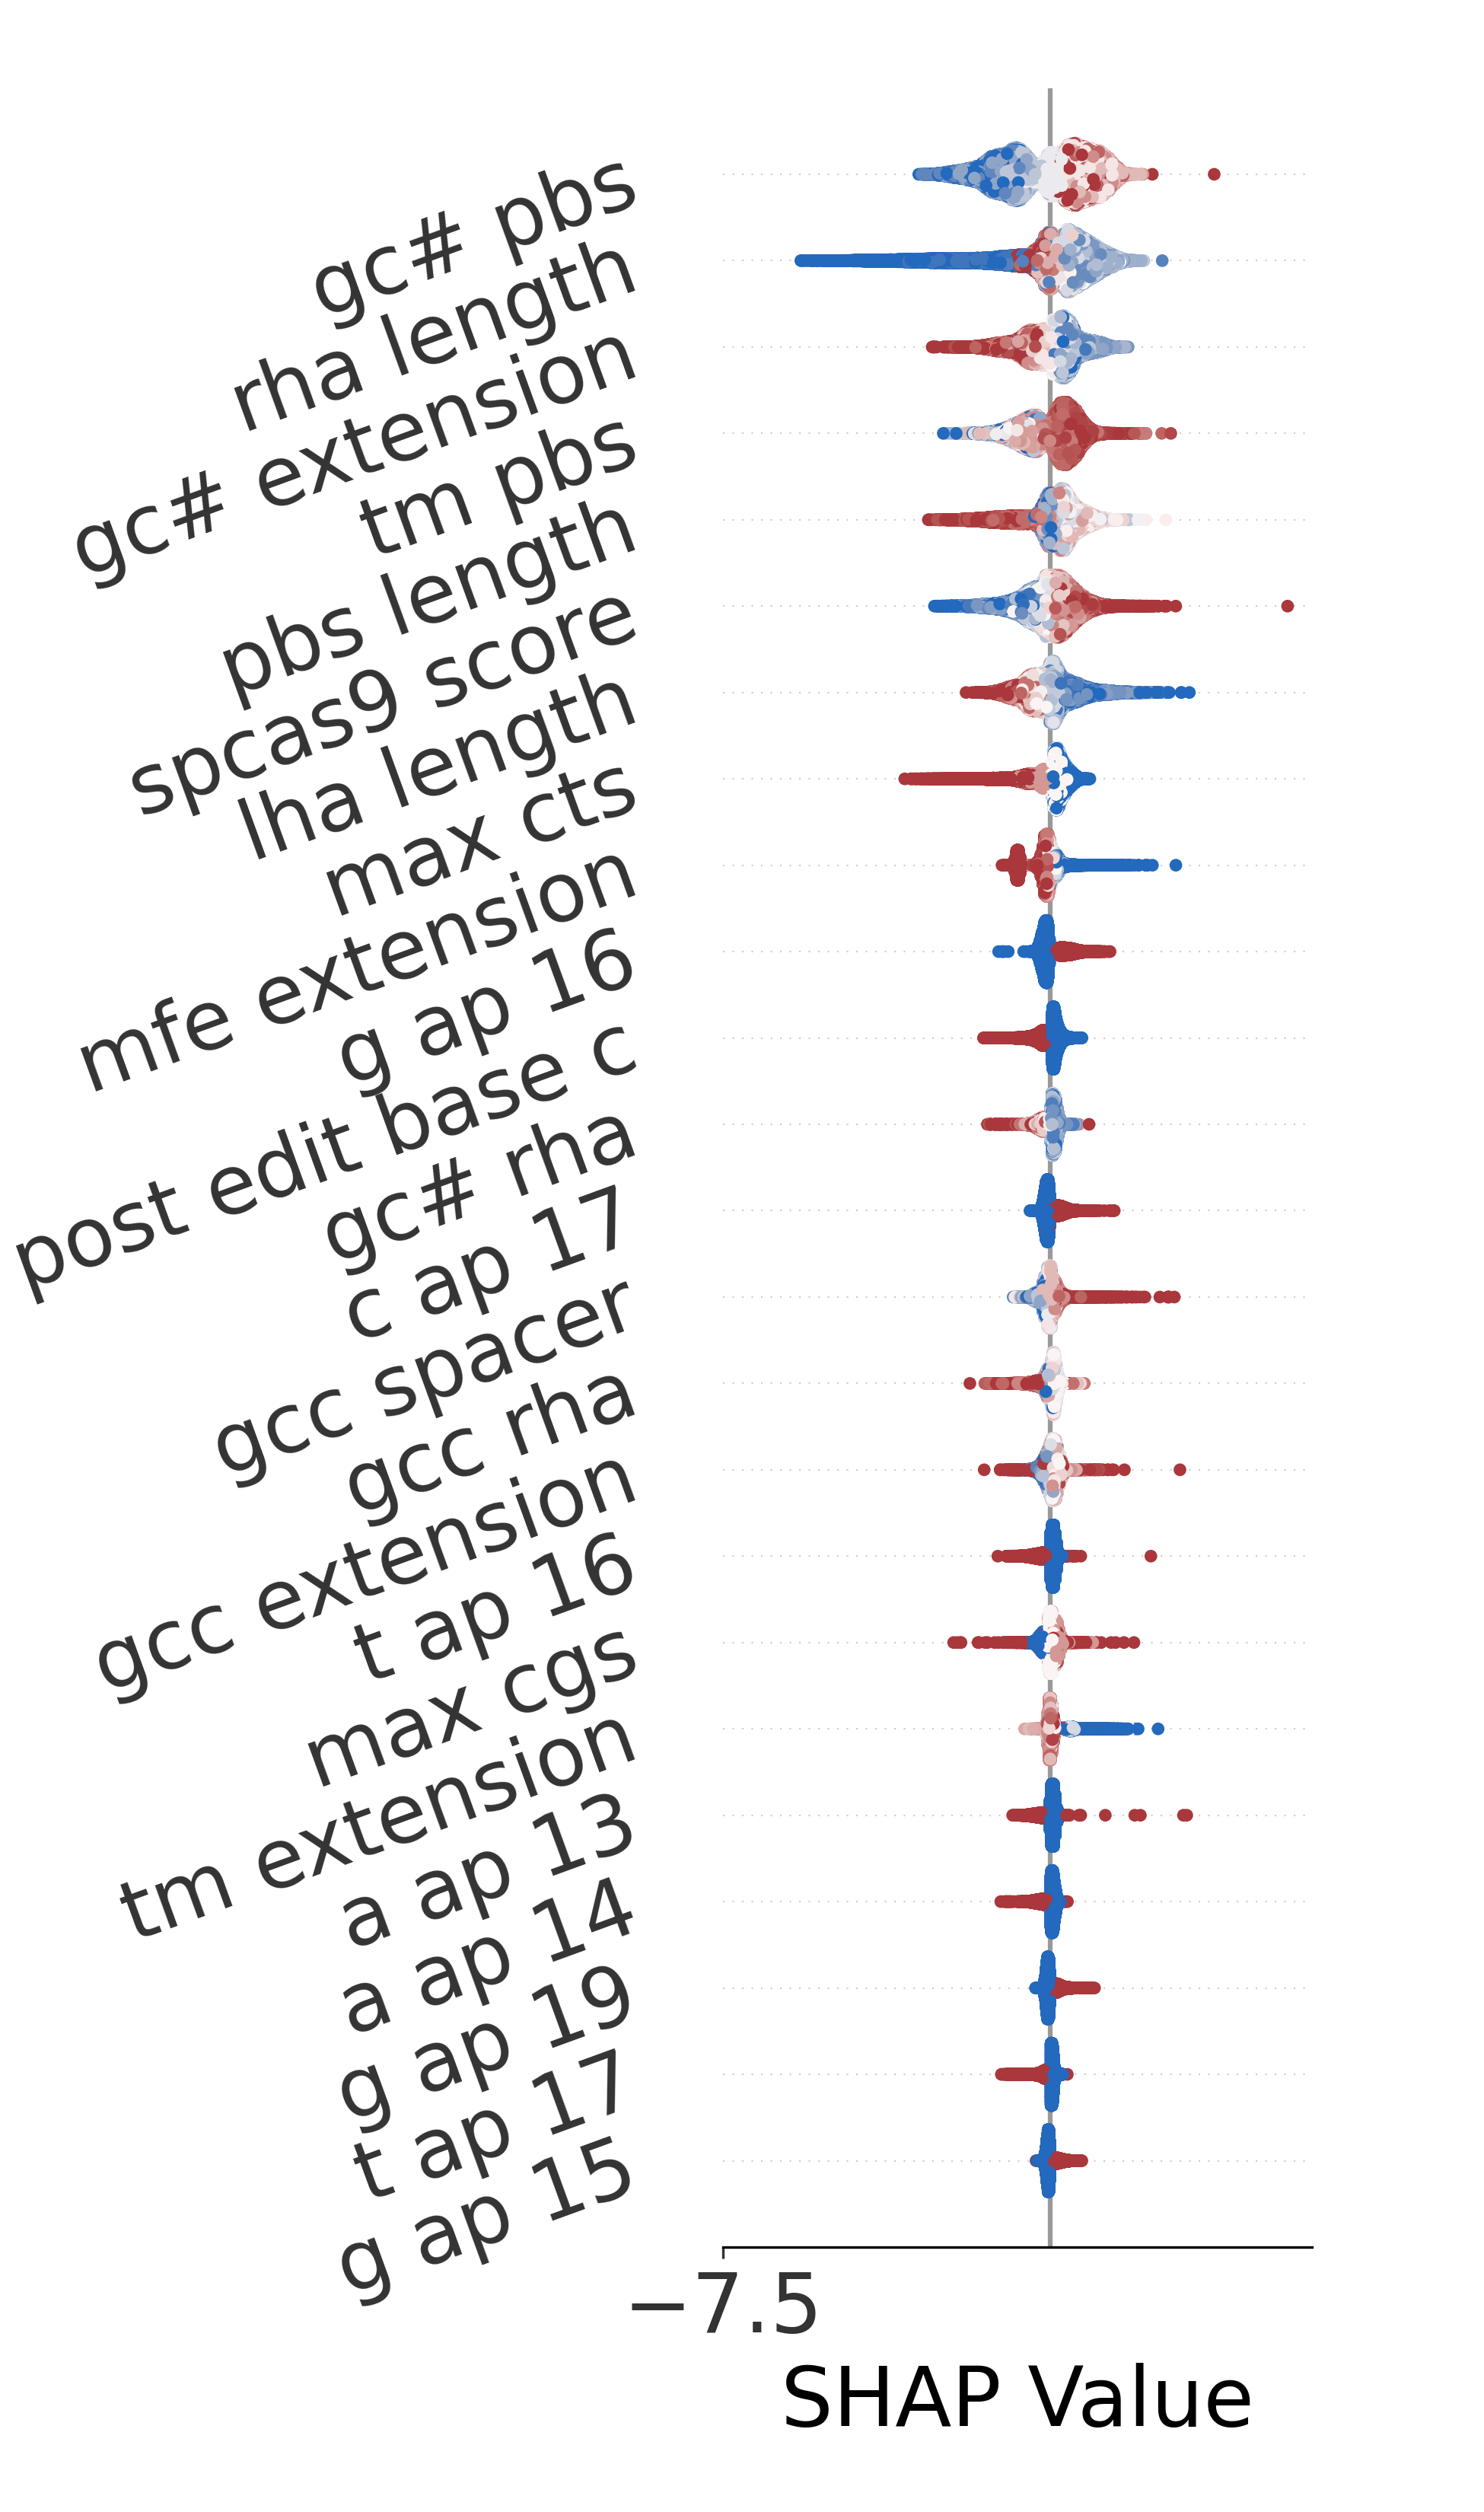
\includegraphics[width=0.3\textwidth]{shap_1bp-dp-hek293t-pe2-replace.png}
        \label{fig:shap_replacement}
    }%
    \subfigure[Insertion]{
        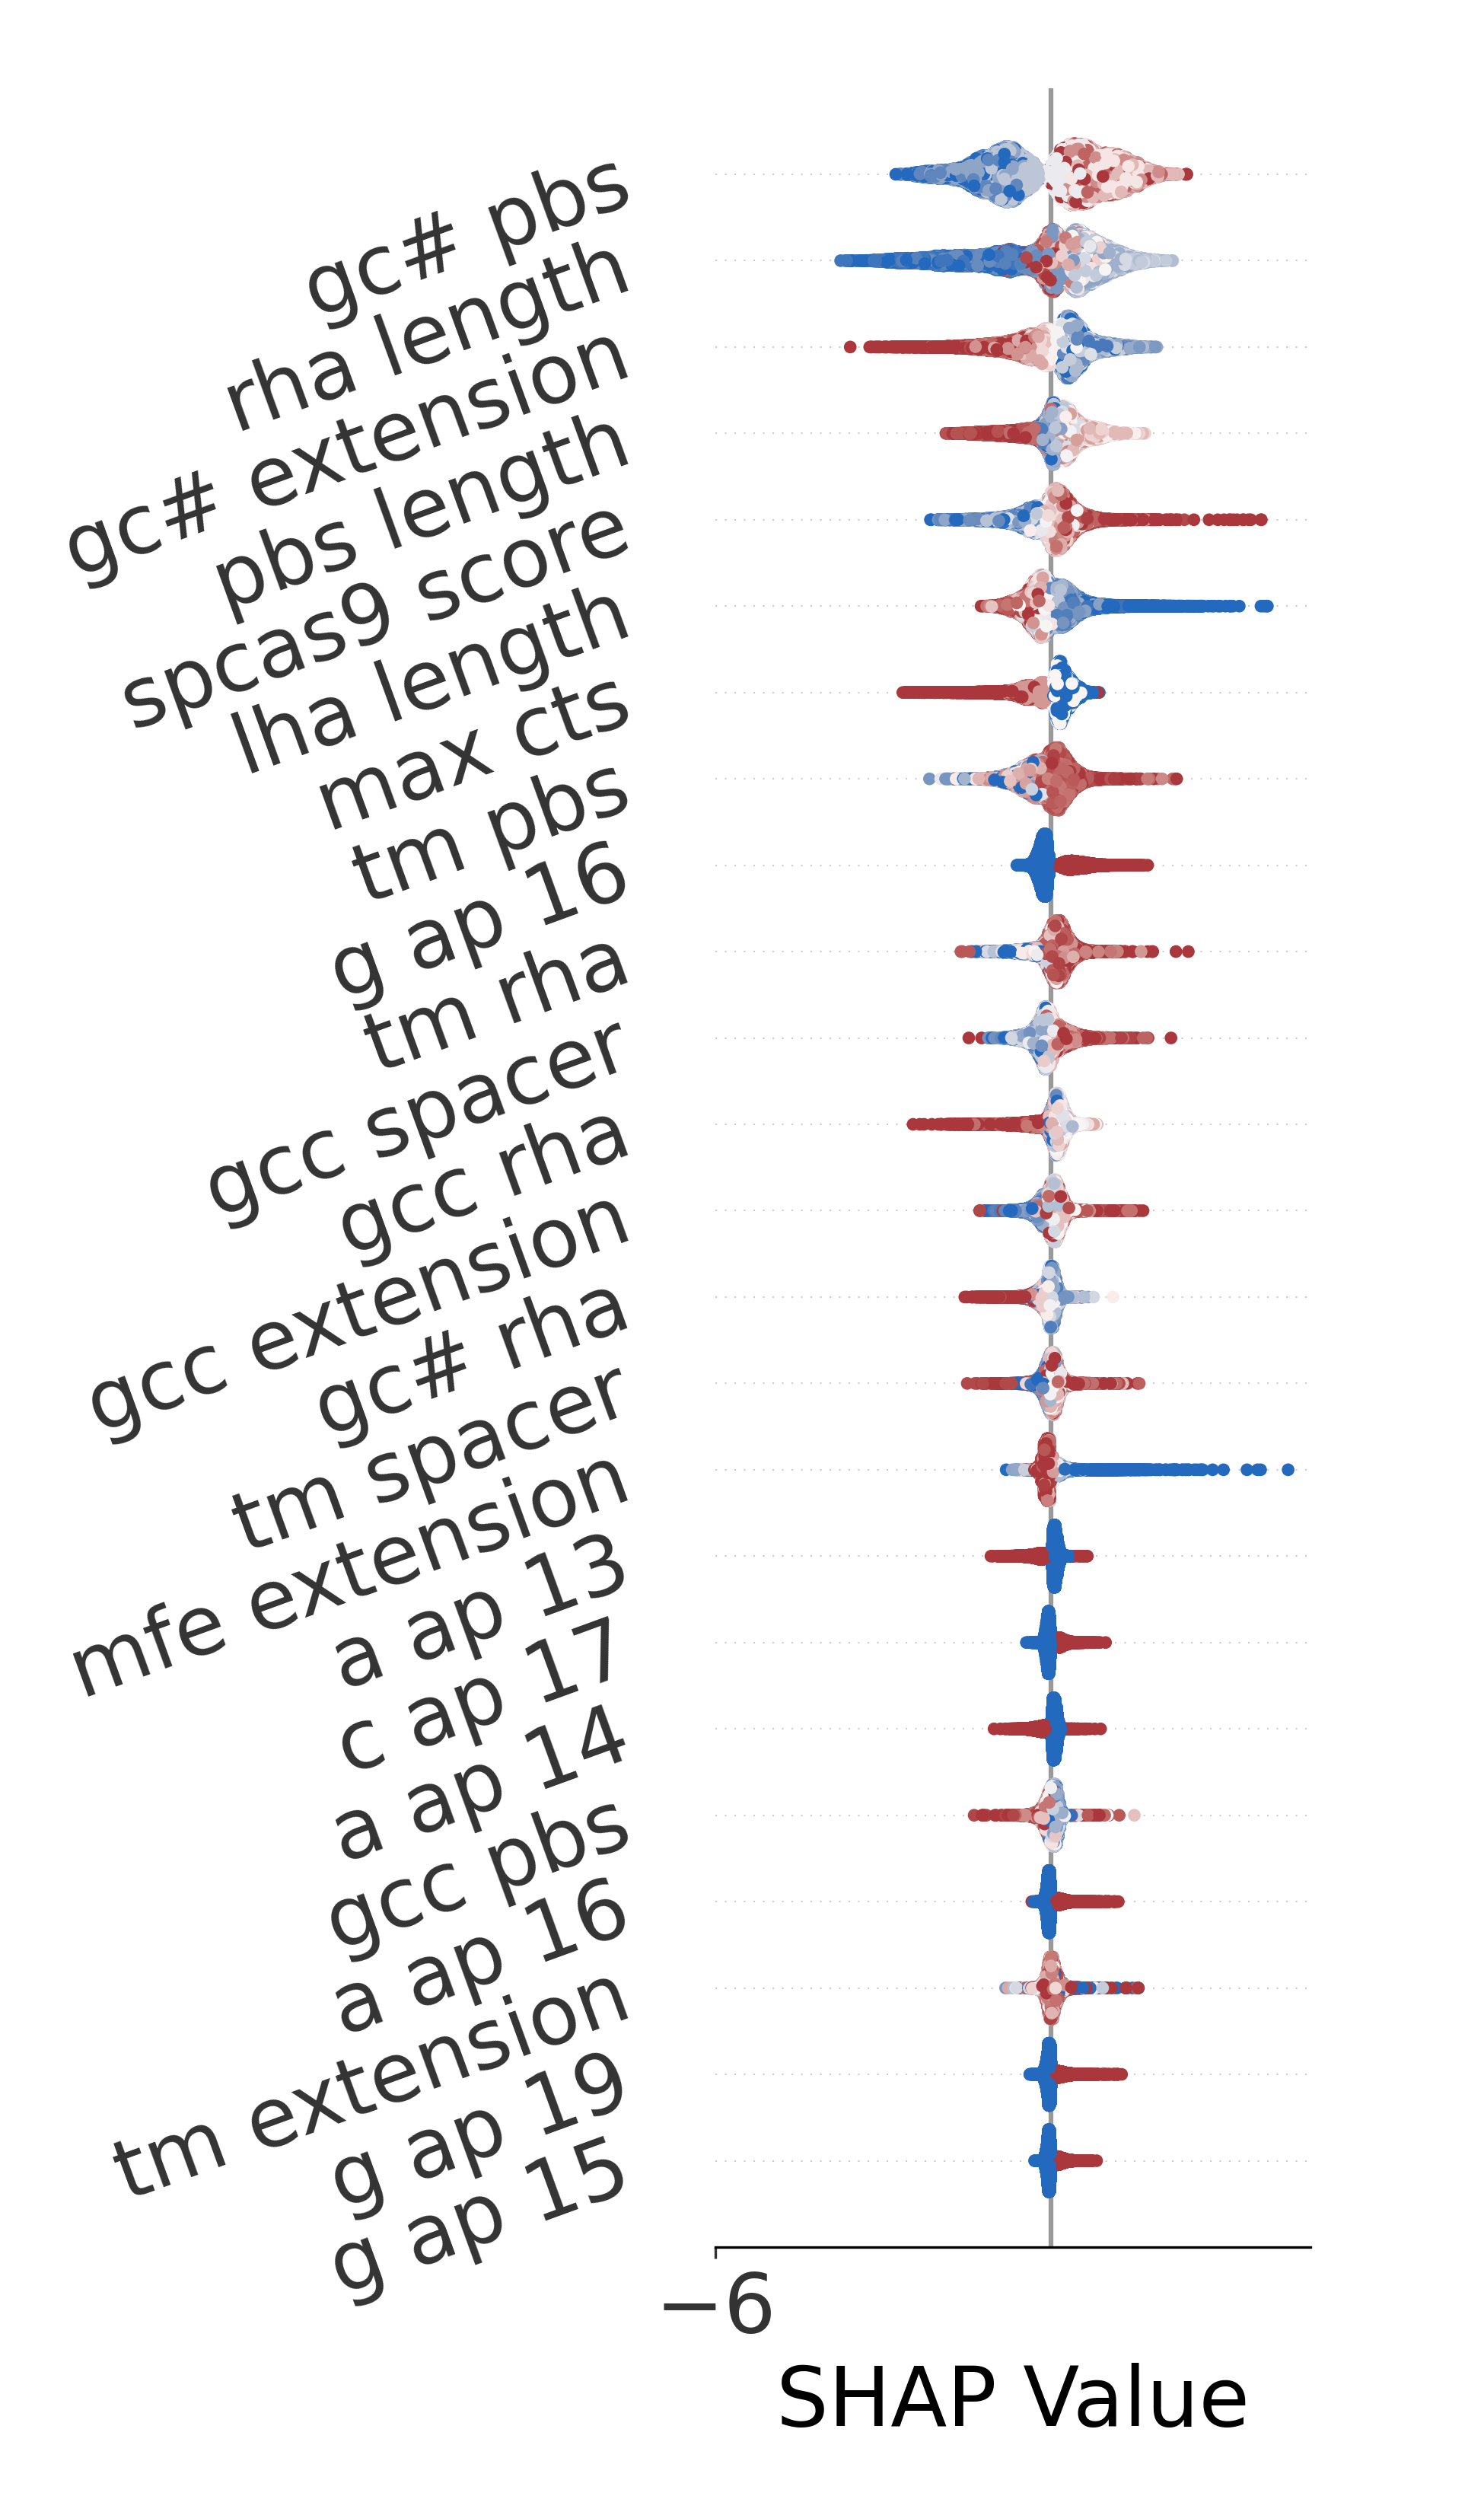
\includegraphics[width=0.3\textwidth]{shap_1bp-dp-hek293t-pe2-insert.png}
        \label{fig:shap_insertion}
    }%
    \subfigure[Deletion]{
        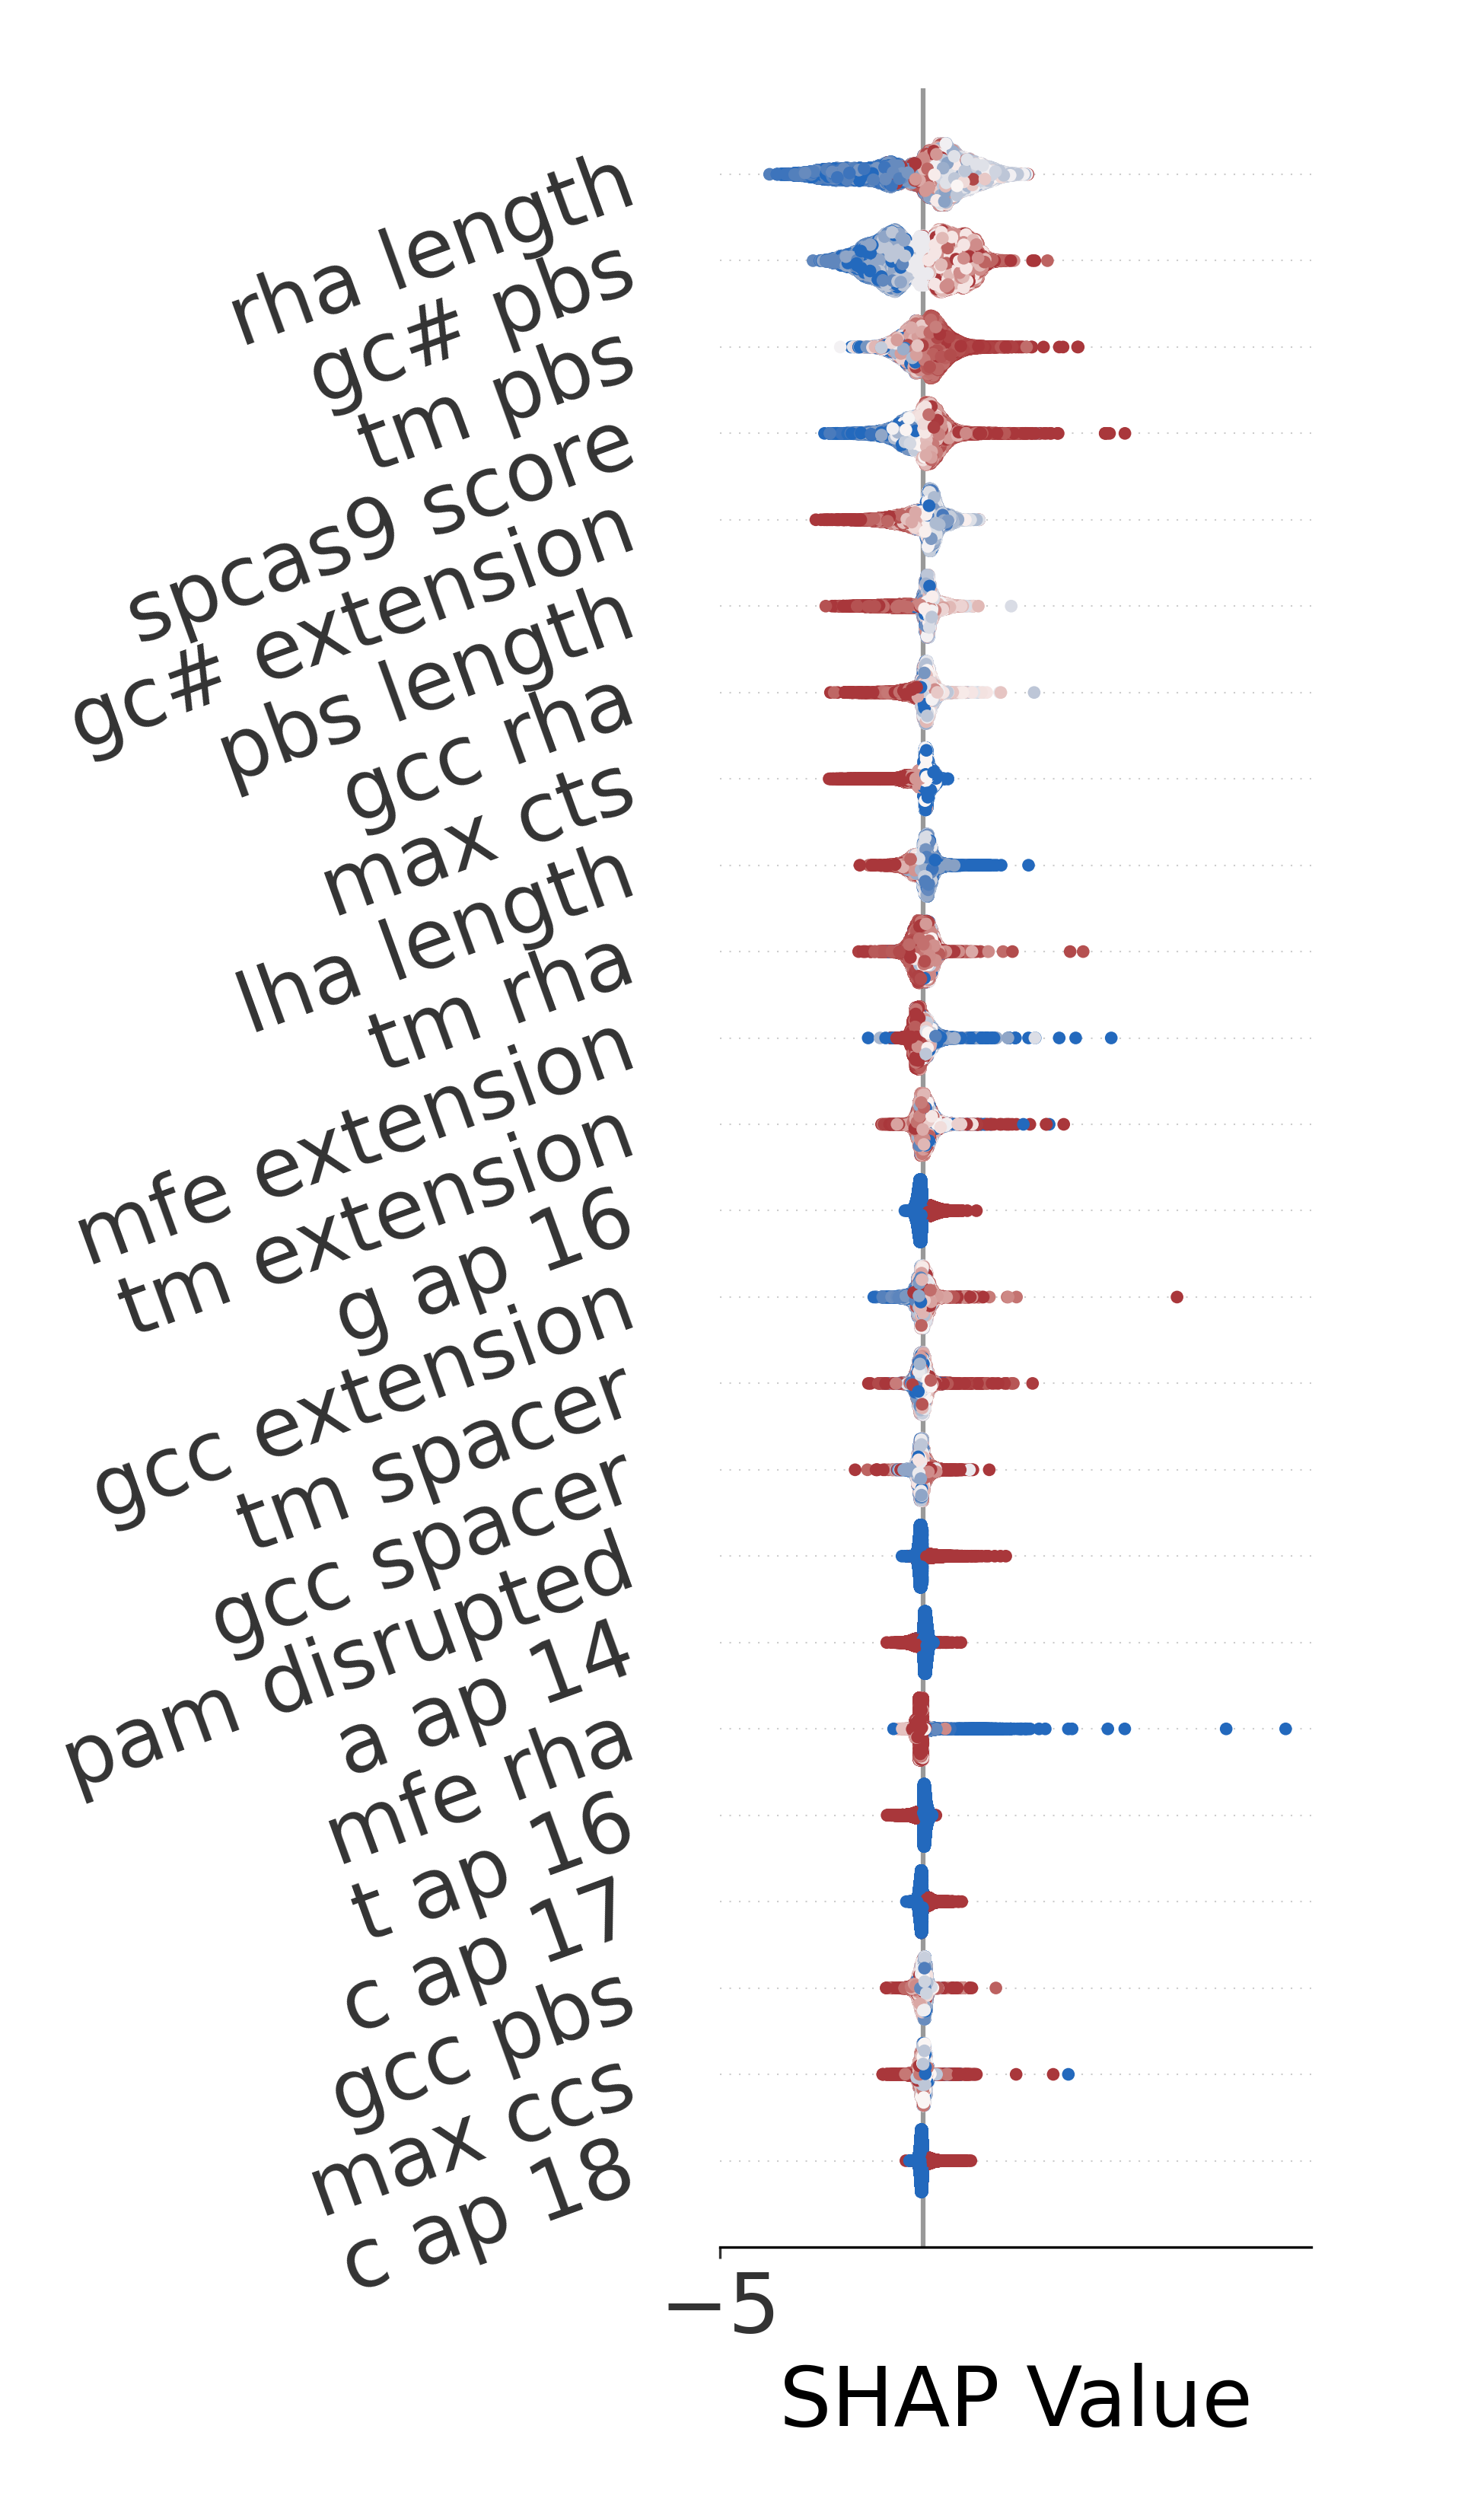
\includegraphics[width=0.3\textwidth]{shap_1bp-dp-hek293t-pe2-delete.png}
        \label{fig:shap_deletion}
    }
    \caption[SHAP analysis for 1-bp insertion and deletion of the DeepPrime model trained on the HEK293T-PE2 dataset]{SHAP analysis for 1-bp insertion and deletion of the DeepPrime model trained on the HEK293T-PE2 dataset. The x-axis represents the attributed weight to the outcome (SHAP value), while the y-axis represents the features ranked by importance (mean absolute SHAP value, highest on top). The colour of the points indicates the feature value, with red indicating high values and blue indicating low values.}
    \label{fig:shap-1bp}
\end{figure}

The attention weights for the edits of length 3 showed similar result (\autoref{fig:attention_deletion_3bp}), the only noticeable difference is that the high attention regions for deletion were extended to 3bp long, reflecting the longer deletion length.

During SHAP analysis in \autoref{sec:determinants}, the edited base was not investigated, as a meaningful representation for bases of different lengths could not be found. Thus, to understand if the base to edit during deletion was indeed an important feature, SHAP analysis was conducted again on the HEK293T PE2 dataset for 1-bp replacement, insertion, and deletion (\autoref{fig:shap-1bp}).

Interestingly, different from the result of attention analysis, the base to edit during deletion was not considered an important feature by the XGBoost model (Figure \ref{fig:shap_deletion}). Consistent results were seen on the four PRIDICT datasets (\autoref{appendix:shap-1bp-pridict}), as well as the A562 PE2-max dataset, where the transformer model significantly outperformed PRIDICT and DeepPrime. This to some extent undermines transformer model's advantage in performance, suggesting that the better correlation could be a result of randomness in the training process, rather than the inherent superiority of the model architecture.